% Created by tikzDevice version 0.12.3.1 on 2022-09-05 08:11:43
% !TEX encoding = UTF-8 Unicode
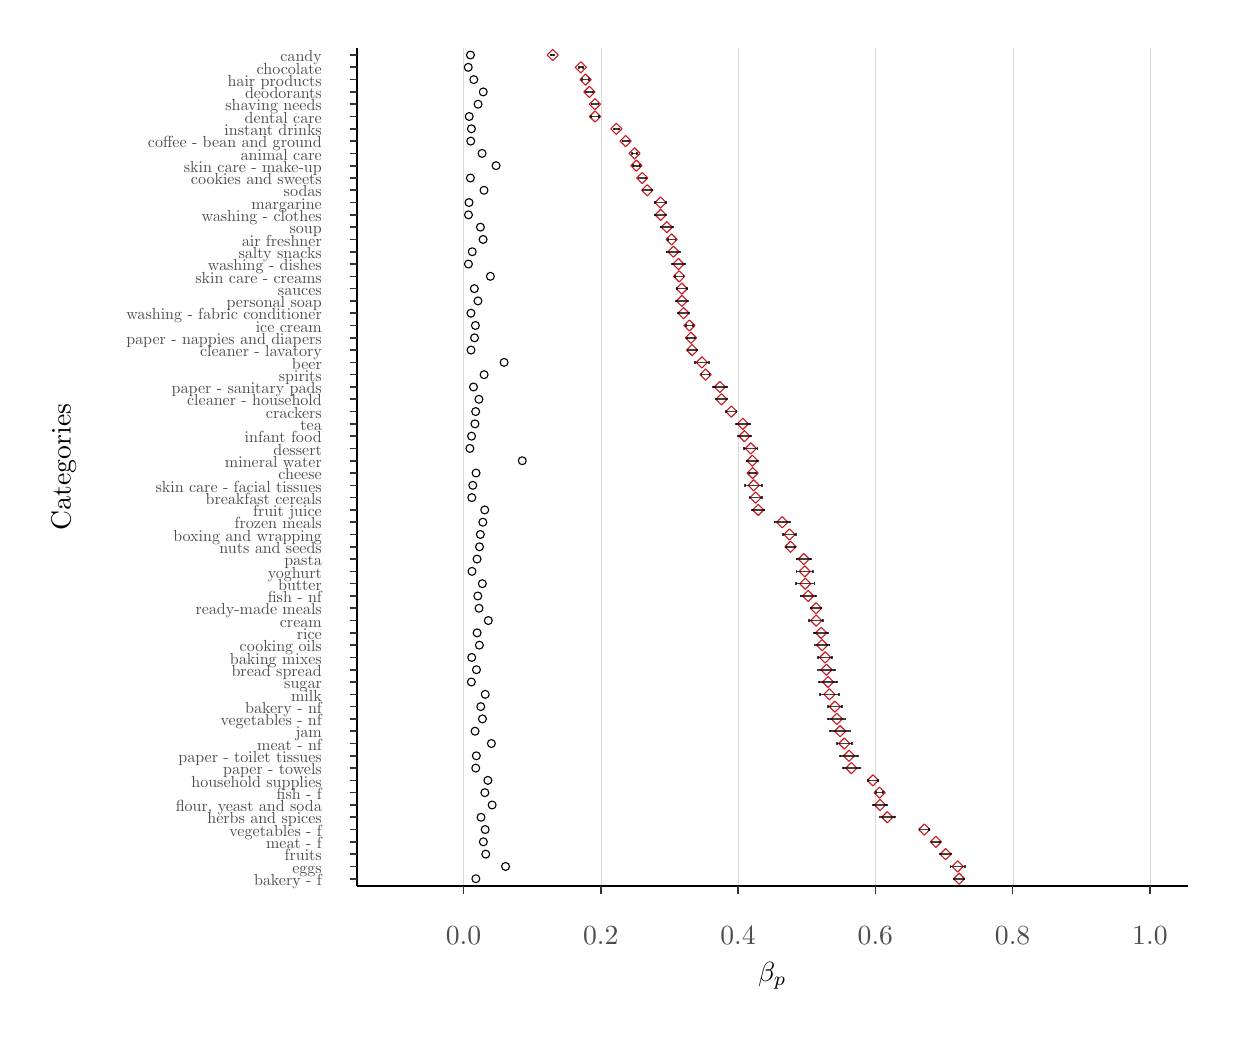
\begin{tikzpicture}[x=1pt,y=1pt]
\definecolor{fillColor}{RGB}{255,255,255}
\path[use as bounding box,fill=fillColor,fill opacity=0.00] (0,0) rectangle (433.62,361.35);
\begin{scope}
\path[clip] (  0.00,  0.00) rectangle (433.62,361.35);
\definecolor{drawColor}{RGB}{255,255,255}
\definecolor{fillColor}{RGB}{255,255,255}

\path[draw=drawColor,line width= 0.6pt,line join=round,line cap=round,fill=fillColor] (  0.00,  0.00) rectangle (433.62,361.35);
\end{scope}
\begin{scope}
\path[clip] (119.04, 51.15) rectangle (419.17,354.12);
\definecolor{drawColor}{RGB}{255,255,255}

\path[draw=drawColor,line width= 0.3pt,line join=round] (132.68, 51.15) --
	(132.68,354.12);

\path[draw=drawColor,line width= 0.3pt,line join=round] (182.29, 51.15) --
	(182.29,354.12);

\path[draw=drawColor,line width= 0.3pt,line join=round] (231.90, 51.15) --
	(231.90,354.12);

\path[draw=drawColor,line width= 0.3pt,line join=round] (281.51, 51.15) --
	(281.51,354.12);

\path[draw=drawColor,line width= 0.3pt,line join=round] (331.11, 51.15) --
	(331.11,354.12);

\path[draw=drawColor,line width= 0.3pt,line join=round] (380.72, 51.15) --
	(380.72,354.12);
\definecolor{drawColor}{gray}{0.85}

\path[draw=drawColor,line width= 0.1pt,line join=round] (157.49, 51.15) --
	(157.49,354.12);

\path[draw=drawColor,line width= 0.1pt,line join=round] (207.09, 51.15) --
	(207.09,354.12);

\path[draw=drawColor,line width= 0.1pt,line join=round] (256.70, 51.15) --
	(256.70,354.12);

\path[draw=drawColor,line width= 0.1pt,line join=round] (306.31, 51.15) --
	(306.31,354.12);

\path[draw=drawColor,line width= 0.1pt,line join=round] (355.92, 51.15) --
	(355.92,354.12);

\path[draw=drawColor,line width= 0.1pt,line join=round] (405.52, 51.15) --
	(405.52,354.12);
\definecolor{drawColor}{RGB}{0,0,0}

\path[draw=drawColor,line width= 0.4pt,line join=round,line cap=round] (164.56,284.82) circle (  1.43);

\path[draw=drawColor,line width= 0.4pt,line join=round,line cap=round] (164.19,315.92) circle (  1.43);

\path[draw=drawColor,line width= 0.4pt,line join=round,line cap=round] (161.95, 53.82) circle (  1.43);

\path[draw=drawColor,line width= 0.4pt,line join=round,line cap=round] (163.72,116.01) circle (  1.43);

\path[draw=drawColor,line width= 0.4pt,line join=round,line cap=round] (160.46,133.78) circle (  1.43);

\path[draw=drawColor,line width= 0.4pt,line join=round,line cap=round] (172.15,240.40) circle (  1.43);

\path[draw=drawColor,line width= 0.4pt,line join=round,line cap=round] (163.57,178.21) circle (  1.43);

\path[draw=drawColor,line width= 0.4pt,line join=round,line cap=round] (162.17,129.34) circle (  1.43);

\path[draw=drawColor,line width= 0.4pt,line join=round,line cap=round] (160.49,191.53) circle (  1.43);

\path[draw=drawColor,line width= 0.4pt,line join=round,line cap=round] (164.29,160.44) circle (  1.43);

\path[draw=drawColor,line width= 0.4pt,line join=round,line cap=round] (159.99,351.46) circle (  1.43);

\path[draw=drawColor,line width= 0.4pt,line join=round,line cap=round] (162.02,200.42) circle (  1.43);

\path[draw=drawColor,line width= 0.4pt,line join=round,line cap=round] (159.20,347.02) circle (  1.43);

\path[draw=drawColor,line width= 0.4pt,line join=round,line cap=round] (163.06,227.07) circle (  1.43);

\path[draw=drawColor,line width= 0.4pt,line join=round,line cap=round] (160.20,244.84) circle (  1.43);

\path[draw=drawColor,line width= 0.4pt,line join=round,line cap=round] (160.10,320.36) circle (  1.43);

\path[draw=drawColor,line width= 0.4pt,line join=round,line cap=round] (159.97,307.03) circle (  1.43);

\path[draw=drawColor,line width= 0.4pt,line join=round,line cap=round] (163.22,138.22) circle (  1.43);

\path[draw=drawColor,line width= 0.4pt,line join=round,line cap=round] (161.88,222.63) circle (  1.43);

\path[draw=drawColor,line width= 0.4pt,line join=round,line cap=round] (166.45,147.11) circle (  1.43);

\path[draw=drawColor,line width= 0.4pt,line join=round,line cap=round] (159.55,329.25) circle (  1.43);

\path[draw=drawColor,line width= 0.4pt,line join=round,line cap=round] (164.61,338.13) circle (  1.43);

\path[draw=drawColor,line width= 0.4pt,line join=round,line cap=round] (159.79,209.30) circle (  1.43);

\path[draw=drawColor,line width= 0.4pt,line join=round,line cap=round] (172.68, 58.26) circle (  1.43);

\path[draw=drawColor,line width= 0.4pt,line join=round,line cap=round] (165.20, 84.92) circle (  1.43);

\path[draw=drawColor,line width= 0.4pt,line join=round,line cap=round] (162.65,155.99) circle (  1.43);

\path[draw=drawColor,line width= 0.4pt,line join=round,line cap=round] (167.83, 80.47) circle (  1.43);

\path[draw=drawColor,line width= 0.4pt,line join=round,line cap=round] (164.47,182.65) circle (  1.43);

\path[draw=drawColor,line width= 0.4pt,line join=round,line cap=round] (165.16,187.09) circle (  1.43);

\path[draw=drawColor,line width= 0.4pt,line join=round,line cap=round] (165.53, 62.70) circle (  1.43);

\path[draw=drawColor,line width= 0.4pt,line join=round,line cap=round] (161.21,342.57) circle (  1.43);

\path[draw=drawColor,line width= 0.4pt,line join=round,line cap=round] (163.81, 76.03) circle (  1.43);

\path[draw=drawColor,line width= 0.4pt,line join=round,line cap=round] (166.29, 89.36) circle (  1.43);

\path[draw=drawColor,line width= 0.4pt,line join=round,line cap=round] (161.78,253.73) circle (  1.43);

\path[draw=drawColor,line width= 0.4pt,line join=round,line cap=round] (160.40,213.74) circle (  1.43);

\path[draw=drawColor,line width= 0.4pt,line join=round,line cap=round] (160.34,324.80) circle (  1.43);

\path[draw=drawColor,line width= 0.4pt,line join=round,line cap=round] (161.66,107.13) circle (  1.43);

\path[draw=drawColor,line width= 0.4pt,line join=round,line cap=round] (159.47,298.15) circle (  1.43);

\path[draw=drawColor,line width= 0.4pt,line join=round,line cap=round] (164.66, 67.15) circle (  1.43);

\path[draw=drawColor,line width= 0.4pt,line join=round,line cap=round] (167.56,102.69) circle (  1.43);

\path[draw=drawColor,line width= 0.4pt,line join=round,line cap=round] (165.34,120.45) circle (  1.43);

\path[draw=drawColor,line width= 0.4pt,line join=round,line cap=round] (178.72,204.86) circle (  1.43);

\path[draw=drawColor,line width= 0.4pt,line join=round,line cap=round] (163.26,173.76) circle (  1.43);

\path[draw=drawColor,line width= 0.4pt,line join=round,line cap=round] (161.47,249.28) circle (  1.43);

\path[draw=drawColor,line width= 0.4pt,line join=round,line cap=round] (161.09,231.51) circle (  1.43);

\path[draw=drawColor,line width= 0.4pt,line join=round,line cap=round] (162.12, 98.24) circle (  1.43);

\path[draw=drawColor,line width= 0.4pt,line join=round,line cap=round] (161.91, 93.80) circle (  1.43);

\path[draw=drawColor,line width= 0.4pt,line join=round,line cap=round] (162.38,169.32) circle (  1.43);

\path[draw=drawColor,line width= 0.4pt,line join=round,line cap=round] (162.71,262.61) circle (  1.43);

\path[draw=drawColor,line width= 0.4pt,line join=round,line cap=round] (163.09,151.55) circle (  1.43);

\path[draw=drawColor,line width= 0.4pt,line join=round,line cap=round] (162.40,142.67) circle (  1.43);

\path[draw=drawColor,line width= 0.4pt,line join=round,line cap=round] (160.64,280.38) circle (  1.43);

\path[draw=drawColor,line width= 0.4pt,line join=round,line cap=round] (161.41,267.05) circle (  1.43);

\path[draw=drawColor,line width= 0.4pt,line join=round,line cap=round] (162.75,333.69) circle (  1.43);

\path[draw=drawColor,line width= 0.4pt,line join=round,line cap=round] (167.20,271.49) circle (  1.43);

\path[draw=drawColor,line width= 0.4pt,line join=round,line cap=round] (160.84,195.97) circle (  1.43);

\path[draw=drawColor,line width= 0.4pt,line join=round,line cap=round] (169.26,311.48) circle (  1.43);

\path[draw=drawColor,line width= 0.4pt,line join=round,line cap=round] (164.89,302.59) circle (  1.43);

\path[draw=drawColor,line width= 0.4pt,line join=round,line cap=round] (163.59,289.26) circle (  1.43);

\path[draw=drawColor,line width= 0.4pt,line join=round,line cap=round] (164.93,235.96) circle (  1.43);

\path[draw=drawColor,line width= 0.4pt,line join=round,line cap=round] (160.33,124.90) circle (  1.43);

\path[draw=drawColor,line width= 0.4pt,line join=round,line cap=round] (161.62,218.19) circle (  1.43);

\path[draw=drawColor,line width= 0.4pt,line join=round,line cap=round] (165.32, 71.59) circle (  1.43);

\path[draw=drawColor,line width= 0.4pt,line join=round,line cap=round] (164.33,111.57) circle (  1.43);

\path[draw=drawColor,line width= 0.4pt,line join=round,line cap=round] (159.28,293.71) circle (  1.43);

\path[draw=drawColor,line width= 0.4pt,line join=round,line cap=round] (159.27,275.94) circle (  1.43);

\path[draw=drawColor,line width= 0.4pt,line join=round,line cap=round] (160.18,258.17) circle (  1.43);

\path[draw=drawColor,line width= 0.4pt,line join=round,line cap=round] (160.55,164.88) circle (  1.43);
\definecolor{drawColor}{RGB}{203,24,29}

\path[draw=drawColor,line width= 0.4pt,line join=round,line cap=round] (230.66,284.82) --
	(232.68,286.84) --
	(234.69,284.82) --
	(232.68,282.80) --
	cycle;

\path[draw=drawColor,line width= 0.4pt,line join=round,line cap=round] (217.27,315.92) --
	(219.28,317.94) --
	(221.30,315.92) --
	(219.28,313.90) --
	cycle;

\path[draw=drawColor,line width= 0.4pt,line join=round,line cap=round] (334.56, 53.82) --
	(336.57, 55.84) --
	(338.59, 53.82) --
	(336.57, 51.80) --
	cycle;

\path[draw=drawColor,line width= 0.4pt,line join=round,line cap=round] (289.70,116.01) --
	(291.71,118.03) --
	(293.73,116.01) --
	(291.71,113.99) --
	cycle;

\path[draw=drawColor,line width= 0.4pt,line join=round,line cap=round] (286.14,133.78) --
	(288.16,135.80) --
	(290.18,133.78) --
	(288.16,131.76) --
	cycle;

\path[draw=drawColor,line width= 0.4pt,line join=round,line cap=round] (241.62,240.40) --
	(243.64,242.42) --
	(245.66,240.40) --
	(243.64,238.38) --
	cycle;

\path[draw=drawColor,line width= 0.4pt,line join=round,line cap=round] (273.27,178.21) --
	(275.29,180.22) --
	(277.30,178.21) --
	(275.29,176.19) --
	cycle;

\path[draw=drawColor,line width= 0.4pt,line join=round,line cap=round] (286.60,129.34) --
	(288.62,131.36) --
	(290.64,129.34) --
	(288.62,127.32) --
	cycle;

\path[draw=drawColor,line width= 0.4pt,line join=round,line cap=round] (261.03,191.53) --
	(263.04,193.55) --
	(265.06,191.53) --
	(263.04,189.51) --
	cycle;

\path[draw=drawColor,line width= 0.4pt,line join=round,line cap=round] (278.96,160.44) --
	(280.98,162.45) --
	(283.00,160.44) --
	(280.98,158.42) --
	cycle;

\path[draw=drawColor,line width= 0.4pt,line join=round,line cap=round] (187.72,351.46) --
	(189.74,353.48) --
	(191.76,351.46) --
	(189.74,349.44) --
	cycle;

\path[draw=drawColor,line width= 0.4pt,line join=round,line cap=round] (259.94,200.42) --
	(261.96,202.43) --
	(263.98,200.42) --
	(261.96,198.40) --
	cycle;

\path[draw=drawColor,line width= 0.4pt,line join=round,line cap=round] (197.85,347.02) --
	(199.87,349.03) --
	(201.88,347.02) --
	(199.87,345.00) --
	cycle;

\path[draw=drawColor,line width= 0.4pt,line join=round,line cap=round] (248.69,227.07) --
	(250.70,229.09) --
	(252.72,227.07) --
	(250.70,225.05) --
	cycle;

\path[draw=drawColor,line width= 0.4pt,line join=round,line cap=round] (238.10,244.84) --
	(240.12,246.86) --
	(242.14,244.84) --
	(240.12,242.82) --
	cycle;

\path[draw=drawColor,line width= 0.4pt,line join=round,line cap=round] (214.07,320.36) --
	(216.09,322.38) --
	(218.11,320.36) --
	(216.09,318.34) --
	cycle;

\path[draw=drawColor,line width= 0.4pt,line join=round,line cap=round] (220.04,307.03) --
	(222.06,309.05) --
	(224.08,307.03) --
	(222.06,305.02) --
	cycle;

\path[draw=drawColor,line width= 0.4pt,line join=round,line cap=round] (285.04,138.22) --
	(287.06,140.24) --
	(289.07,138.22) --
	(287.06,136.21) --
	cycle;

\path[draw=drawColor,line width= 0.4pt,line join=round,line cap=round] (252.26,222.63) --
	(254.27,224.65) --
	(256.29,222.63) --
	(254.27,220.61) --
	cycle;

\path[draw=drawColor,line width= 0.4pt,line join=round,line cap=round] (282.90,147.11) --
	(284.92,149.13) --
	(286.93,147.11) --
	(284.92,145.09) --
	cycle;

\path[draw=drawColor,line width= 0.4pt,line join=round,line cap=round] (203.00,329.25) --
	(205.02,331.26) --
	(207.04,329.25) --
	(205.02,327.23) --
	cycle;

\path[draw=drawColor,line width= 0.4pt,line join=round,line cap=round] (200.97,338.13) --
	(202.99,340.15) --
	(205.00,338.13) --
	(202.99,336.11) --
	cycle;

\path[draw=drawColor,line width= 0.4pt,line join=round,line cap=round] (259.31,209.30) --
	(261.33,211.32) --
	(263.35,209.30) --
	(261.33,207.28) --
	cycle;

\path[draw=drawColor,line width= 0.4pt,line join=round,line cap=round] (334.05, 58.26) --
	(336.06, 60.28) --
	(338.08, 58.26) --
	(336.06, 56.24) --
	cycle;

\path[draw=drawColor,line width= 0.4pt,line join=round,line cap=round] (305.81, 84.92) --
	(307.82, 86.93) --
	(309.84, 84.92) --
	(307.82, 82.90) --
	cycle;

\path[draw=drawColor,line width= 0.4pt,line join=round,line cap=round] (280.01,155.99) --
	(282.03,158.01) --
	(284.04,155.99) --
	(282.03,153.98) --
	cycle;

\path[draw=drawColor,line width= 0.4pt,line join=round,line cap=round] (305.98, 80.47) --
	(307.99, 82.49) --
	(310.01, 80.47) --
	(307.99, 78.46) --
	cycle;

\path[draw=drawColor,line width= 0.4pt,line join=round,line cap=round] (270.64,182.65) --
	(272.66,184.67) --
	(274.68,182.65) --
	(272.66,180.63) --
	cycle;

\path[draw=drawColor,line width= 0.4pt,line join=round,line cap=round] (261.98,187.09) --
	(264.00,189.11) --
	(266.02,187.09) --
	(264.00,185.07) --
	cycle;

\path[draw=drawColor,line width= 0.4pt,line join=round,line cap=round] (329.70, 62.70) --
	(331.72, 64.72) --
	(333.74, 62.70) --
	(331.72, 60.69) --
	cycle;

\path[draw=drawColor,line width= 0.4pt,line join=round,line cap=round] (199.57,342.57) --
	(201.59,344.59) --
	(203.61,342.57) --
	(201.59,340.56) --
	cycle;

\path[draw=drawColor,line width= 0.4pt,line join=round,line cap=round] (308.61, 76.03) --
	(310.63, 78.05) --
	(312.64, 76.03) --
	(310.63, 74.01) --
	cycle;

\path[draw=drawColor,line width= 0.4pt,line join=round,line cap=round] (303.43, 89.36) --
	(305.45, 91.38) --
	(307.47, 89.36) --
	(305.45, 87.34) --
	cycle;

\path[draw=drawColor,line width= 0.4pt,line join=round,line cap=round] (237.11,253.73) --
	(239.12,255.74) --
	(241.14,253.73) --
	(239.12,251.71) --
	cycle;

\path[draw=drawColor,line width= 0.4pt,line join=round,line cap=round] (256.99,213.74) --
	(259.00,215.76) --
	(261.02,213.74) --
	(259.00,211.73) --
	cycle;

\path[draw=drawColor,line width= 0.4pt,line join=round,line cap=round] (210.69,324.80) --
	(212.71,326.82) --
	(214.73,324.80) --
	(212.71,322.79) --
	cycle;

\path[draw=drawColor,line width= 0.4pt,line join=round,line cap=round] (291.56,107.13) --
	(293.58,109.14) --
	(295.60,107.13) --
	(293.58,105.11) --
	cycle;

\path[draw=drawColor,line width= 0.4pt,line join=round,line cap=round] (226.67,298.15) --
	(228.69,300.17) --
	(230.71,298.15) --
	(228.69,296.13) --
	cycle;

\path[draw=drawColor,line width= 0.4pt,line join=round,line cap=round] (326.13, 67.15) --
	(328.15, 69.16) --
	(330.17, 67.15) --
	(328.15, 65.13) --
	cycle;

\path[draw=drawColor,line width= 0.4pt,line join=round,line cap=round] (293.07,102.69) --
	(295.09,104.70) --
	(297.11,102.69) --
	(295.09,100.67) --
	cycle;

\path[draw=drawColor,line width= 0.4pt,line join=round,line cap=round] (287.70,120.45) --
	(289.72,122.47) --
	(291.74,120.45) --
	(289.72,118.44) --
	cycle;

\path[draw=drawColor,line width= 0.4pt,line join=round,line cap=round] (259.85,204.86) --
	(261.86,206.88) --
	(263.88,204.86) --
	(261.86,202.84) --
	cycle;

\path[draw=drawColor,line width= 0.4pt,line join=round,line cap=round] (273.64,173.76) --
	(275.66,175.78) --
	(277.68,173.76) --
	(275.66,171.75) --
	cycle;

\path[draw=drawColor,line width= 0.4pt,line join=round,line cap=round] (237.66,249.28) --
	(239.68,251.30) --
	(241.70,249.28) --
	(239.68,247.27) --
	cycle;

\path[draw=drawColor,line width= 0.4pt,line join=round,line cap=round] (248.10,231.51) --
	(250.12,233.53) --
	(252.13,231.51) --
	(250.12,229.50) --
	cycle;

\path[draw=drawColor,line width= 0.4pt,line join=round,line cap=round] (294.77, 98.24) --
	(296.79,100.26) --
	(298.80, 98.24) --
	(296.79, 96.23) --
	cycle;

\path[draw=drawColor,line width= 0.4pt,line join=round,line cap=round] (295.64, 93.80) --
	(297.65, 95.82) --
	(299.67, 93.80) --
	(297.65, 91.78) --
	cycle;

\path[draw=drawColor,line width= 0.4pt,line join=round,line cap=round] (278.40,169.32) --
	(280.42,171.34) --
	(282.44,169.32) --
	(280.42,167.30) --
	cycle;

\path[draw=drawColor,line width= 0.4pt,line join=round,line cap=round] (234.39,262.61) --
	(236.41,264.63) --
	(238.42,262.61) --
	(236.41,260.59) --
	cycle;

\path[draw=drawColor,line width= 0.4pt,line join=round,line cap=round] (282.86,151.55) --
	(284.88,153.57) --
	(286.90,151.55) --
	(284.88,149.53) --
	cycle;

\path[draw=drawColor,line width= 0.4pt,line join=round,line cap=round] (284.71,142.67) --
	(286.73,144.68) --
	(288.75,142.67) --
	(286.73,140.65) --
	cycle;

\path[draw=drawColor,line width= 0.4pt,line join=round,line cap=round] (231.31,280.38) --
	(233.33,282.40) --
	(235.34,280.38) --
	(233.33,278.36) --
	cycle;

\path[draw=drawColor,line width= 0.4pt,line join=round,line cap=round] (234.34,267.05) --
	(236.36,269.07) --
	(238.38,267.05) --
	(236.36,265.04) --
	cycle;

\path[draw=drawColor,line width= 0.4pt,line join=round,line cap=round] (202.96,333.69) --
	(204.98,335.71) --
	(206.99,333.69) --
	(204.98,331.67) --
	cycle;

\path[draw=drawColor,line width= 0.4pt,line join=round,line cap=round] (233.41,271.49) --
	(235.42,273.51) --
	(237.44,271.49) --
	(235.42,269.48) --
	cycle;

\path[draw=drawColor,line width= 0.4pt,line join=round,line cap=round] (260.34,195.97) --
	(262.36,197.99) --
	(264.37,195.97) --
	(262.36,193.96) --
	cycle;

\path[draw=drawColor,line width= 0.4pt,line join=round,line cap=round] (217.93,311.48) --
	(219.95,313.49) --
	(221.97,311.48) --
	(219.95,309.46) --
	cycle;

\path[draw=drawColor,line width= 0.4pt,line join=round,line cap=round] (221.87,302.59) --
	(223.88,304.61) --
	(225.90,302.59) --
	(223.88,300.57) --
	cycle;

\path[draw=drawColor,line width= 0.4pt,line join=round,line cap=round] (228.92,289.26) --
	(230.94,291.28) --
	(232.96,289.26) --
	(230.94,287.25) --
	cycle;

\path[draw=drawColor,line width= 0.4pt,line join=round,line cap=round] (242.94,235.96) --
	(244.96,237.97) --
	(246.98,235.96) --
	(244.96,233.94) --
	cycle;

\path[draw=drawColor,line width= 0.4pt,line join=round,line cap=round] (287.21,124.90) --
	(289.23,126.91) --
	(291.25,124.90) --
	(289.23,122.88) --
	cycle;

\path[draw=drawColor,line width= 0.4pt,line join=round,line cap=round] (256.40,218.19) --
	(258.42,220.20) --
	(260.44,218.19) --
	(258.42,216.17) --
	cycle;

\path[draw=drawColor,line width= 0.4pt,line join=round,line cap=round] (321.96, 71.59) --
	(323.98, 73.61) --
	(326.00, 71.59) --
	(323.98, 69.57) --
	cycle;

\path[draw=drawColor,line width= 0.4pt,line join=round,line cap=round] (290.39,111.57) --
	(292.40,113.59) --
	(294.42,111.57) --
	(292.40,109.55) --
	cycle;

\path[draw=drawColor,line width= 0.4pt,line join=round,line cap=round] (226.72,293.71) --
	(228.74,295.72) --
	(230.76,293.71) --
	(228.74,291.69) --
	cycle;

\path[draw=drawColor,line width= 0.4pt,line join=round,line cap=round] (233.14,275.94) --
	(235.16,277.95) --
	(237.17,275.94) --
	(235.16,273.92) --
	cycle;

\path[draw=drawColor,line width= 0.4pt,line join=round,line cap=round] (234.99,258.17) --
	(237.01,260.19) --
	(239.03,258.17) --
	(237.01,256.15) --
	cycle;

\path[draw=drawColor,line width= 0.4pt,line join=round,line cap=round] (278.78,164.88) --
	(280.80,166.90) --
	(282.81,164.88) --
	(280.80,162.86) --
	cycle;
\definecolor{drawColor}{RGB}{0,0,0}

\path[draw=drawColor,draw opacity=0.75,line width= 0.6pt,line join=round] (234.07,284.38) --
	(234.07,285.27);

\path[draw=drawColor,draw opacity=0.75,line width= 0.6pt,line join=round] (234.07,284.82) --
	(231.29,284.82);

\path[draw=drawColor,draw opacity=0.75,line width= 0.6pt,line join=round] (231.29,284.38) --
	(231.29,285.27);

\path[draw=drawColor,draw opacity=0.75,line width= 0.6pt,line join=round] (220.14,315.47) --
	(220.14,316.36);

\path[draw=drawColor,draw opacity=0.75,line width= 0.6pt,line join=round] (220.14,315.92) --
	(218.42,315.92);

\path[draw=drawColor,draw opacity=0.75,line width= 0.6pt,line join=round] (218.42,315.47) --
	(218.42,316.36);

\path[draw=drawColor,draw opacity=0.75,line width= 0.6pt,line join=round] (338.35, 53.37) --
	(338.35, 54.26);

\path[draw=drawColor,draw opacity=0.75,line width= 0.6pt,line join=round] (338.35, 53.82) --
	(334.80, 53.82);

\path[draw=drawColor,draw opacity=0.75,line width= 0.6pt,line join=round] (334.80, 53.37) --
	(334.80, 54.26);

\path[draw=drawColor,draw opacity=0.75,line width= 0.6pt,line join=round] (294.18,115.57) --
	(294.18,116.46);

\path[draw=drawColor,draw opacity=0.75,line width= 0.6pt,line join=round] (294.18,116.01) --
	(289.25,116.01);

\path[draw=drawColor,draw opacity=0.75,line width= 0.6pt,line join=round] (289.25,115.57) --
	(289.25,116.46);

\path[draw=drawColor,draw opacity=0.75,line width= 0.6pt,line join=round] (290.69,133.34) --
	(290.69,134.23);

\path[draw=drawColor,draw opacity=0.75,line width= 0.6pt,line join=round] (290.69,133.78) --
	(285.63,133.78);

\path[draw=drawColor,draw opacity=0.75,line width= 0.6pt,line join=round] (285.63,133.34) --
	(285.63,134.23);

\path[draw=drawColor,draw opacity=0.75,line width= 0.6pt,line join=round] (246.21,239.95) --
	(246.21,240.84);

\path[draw=drawColor,draw opacity=0.75,line width= 0.6pt,line join=round] (246.21,240.40) --
	(241.07,240.40);

\path[draw=drawColor,draw opacity=0.75,line width= 0.6pt,line join=round] (241.07,239.95) --
	(241.07,240.84);

\path[draw=drawColor,draw opacity=0.75,line width= 0.6pt,line join=round] (277.69,177.76) --
	(277.69,178.65);

\path[draw=drawColor,draw opacity=0.75,line width= 0.6pt,line join=round] (277.69,178.21) --
	(272.88,178.21);

\path[draw=drawColor,draw opacity=0.75,line width= 0.6pt,line join=round] (272.88,177.76) --
	(272.88,178.65);

\path[draw=drawColor,draw opacity=0.75,line width= 0.6pt,line join=round] (291.83,128.90) --
	(291.83,129.78);

\path[draw=drawColor,draw opacity=0.75,line width= 0.6pt,line join=round] (291.83,129.34) --
	(285.41,129.34);

\path[draw=drawColor,draw opacity=0.75,line width= 0.6pt,line join=round] (285.41,128.90) --
	(285.41,129.78);

\path[draw=drawColor,draw opacity=0.75,line width= 0.6pt,line join=round] (265.30,191.09) --
	(265.30,191.98);

\path[draw=drawColor,draw opacity=0.75,line width= 0.6pt,line join=round] (265.30,191.53) --
	(260.79,191.53);

\path[draw=drawColor,draw opacity=0.75,line width= 0.6pt,line join=round] (260.79,191.09) --
	(260.79,191.98);

\path[draw=drawColor,draw opacity=0.75,line width= 0.6pt,line join=round] (284.26,159.99) --
	(284.26,160.88);

\path[draw=drawColor,draw opacity=0.75,line width= 0.6pt,line join=round] (284.26,160.44) --
	(277.70,160.44);

\path[draw=drawColor,draw opacity=0.75,line width= 0.6pt,line join=round] (277.70,159.99) --
	(277.70,160.88);

\path[draw=drawColor,draw opacity=0.75,line width= 0.6pt,line join=round] (190.27,351.01) --
	(190.27,351.90);

\path[draw=drawColor,draw opacity=0.75,line width= 0.6pt,line join=round] (190.27,351.46) --
	(189.22,351.46);

\path[draw=drawColor,draw opacity=0.75,line width= 0.6pt,line join=round] (189.22,351.01) --
	(189.22,351.90);

\path[draw=drawColor,draw opacity=0.75,line width= 0.6pt,line join=round] (263.17,199.97) --
	(263.17,200.86);

\path[draw=drawColor,draw opacity=0.75,line width= 0.6pt,line join=round] (263.17,200.42) --
	(260.75,200.42);

\path[draw=drawColor,draw opacity=0.75,line width= 0.6pt,line join=round] (260.75,199.97) --
	(260.75,200.86);

\path[draw=drawColor,draw opacity=0.75,line width= 0.6pt,line join=round] (200.55,346.57) --
	(200.55,347.46);

\path[draw=drawColor,draw opacity=0.75,line width= 0.6pt,line join=round] (200.55,347.02) --
	(199.18,347.02);

\path[draw=drawColor,draw opacity=0.75,line width= 0.6pt,line join=round] (199.18,346.57) --
	(199.18,347.46);

\path[draw=drawColor,draw opacity=0.75,line width= 0.6pt,line join=round] (252.67,226.63) --
	(252.67,227.52);

\path[draw=drawColor,draw opacity=0.75,line width= 0.6pt,line join=round] (252.67,227.07) --
	(248.74,227.07);

\path[draw=drawColor,draw opacity=0.75,line width= 0.6pt,line join=round] (248.74,226.63) --
	(248.74,227.52);

\path[draw=drawColor,draw opacity=0.75,line width= 0.6pt,line join=round] (241.86,244.40) --
	(241.86,245.29);

\path[draw=drawColor,draw opacity=0.75,line width= 0.6pt,line join=round] (241.86,244.84) --
	(238.38,244.84);

\path[draw=drawColor,draw opacity=0.75,line width= 0.6pt,line join=round] (238.38,244.40) --
	(238.38,245.29);

\path[draw=drawColor,draw opacity=0.75,line width= 0.6pt,line join=round] (217.30,319.92) --
	(217.30,320.81);

\path[draw=drawColor,draw opacity=0.75,line width= 0.6pt,line join=round] (217.30,320.36) --
	(214.88,320.36);

\path[draw=drawColor,draw opacity=0.75,line width= 0.6pt,line join=round] (214.88,319.92) --
	(214.88,320.81);

\path[draw=drawColor,draw opacity=0.75,line width= 0.6pt,line join=round] (223.38,306.59) --
	(223.38,307.48);

\path[draw=drawColor,draw opacity=0.75,line width= 0.6pt,line join=round] (223.38,307.03) --
	(220.74,307.03);

\path[draw=drawColor,draw opacity=0.75,line width= 0.6pt,line join=round] (220.74,306.59) --
	(220.74,307.48);

\path[draw=drawColor,draw opacity=0.75,line width= 0.6pt,line join=round] (289.76,137.78) --
	(289.76,138.67);

\path[draw=drawColor,draw opacity=0.75,line width= 0.6pt,line join=round] (289.76,138.22) --
	(284.35,138.22);

\path[draw=drawColor,draw opacity=0.75,line width= 0.6pt,line join=round] (284.35,137.78) --
	(284.35,138.67);

\path[draw=drawColor,draw opacity=0.75,line width= 0.6pt,line join=round] (256.10,222.18) --
	(256.10,223.07);

\path[draw=drawColor,draw opacity=0.75,line width= 0.6pt,line join=round] (256.10,222.63) --
	(252.45,222.63);

\path[draw=drawColor,draw opacity=0.75,line width= 0.6pt,line join=round] (252.45,222.18) --
	(252.45,223.07);

\path[draw=drawColor,draw opacity=0.75,line width= 0.6pt,line join=round] (287.43,146.66) --
	(287.43,147.55);

\path[draw=drawColor,draw opacity=0.75,line width= 0.6pt,line join=round] (287.43,147.11) --
	(282.41,147.11);

\path[draw=drawColor,draw opacity=0.75,line width= 0.6pt,line join=round] (282.41,146.66) --
	(282.41,147.55);

\path[draw=drawColor,draw opacity=0.75,line width= 0.6pt,line join=round] (206.40,328.80) --
	(206.40,329.69);

\path[draw=drawColor,draw opacity=0.75,line width= 0.6pt,line join=round] (206.40,329.25) --
	(203.63,329.25);

\path[draw=drawColor,draw opacity=0.75,line width= 0.6pt,line join=round] (203.63,328.80) --
	(203.63,329.69);

\path[draw=drawColor,draw opacity=0.75,line width= 0.6pt,line join=round] (204.24,337.69) --
	(204.24,338.57);

\path[draw=drawColor,draw opacity=0.75,line width= 0.6pt,line join=round] (204.24,338.13) --
	(201.73,338.13);

\path[draw=drawColor,draw opacity=0.75,line width= 0.6pt,line join=round] (201.73,337.69) --
	(201.73,338.57);

\path[draw=drawColor,draw opacity=0.75,line width= 0.6pt,line join=round] (263.74,208.86) --
	(263.74,209.75);

\path[draw=drawColor,draw opacity=0.75,line width= 0.6pt,line join=round] (263.74,209.30) --
	(258.92,209.30);

\path[draw=drawColor,draw opacity=0.75,line width= 0.6pt,line join=round] (258.92,208.86) --
	(258.92,209.75);

\path[draw=drawColor,draw opacity=0.75,line width= 0.6pt,line join=round] (338.68, 57.82) --
	(338.68, 58.71);

\path[draw=drawColor,draw opacity=0.75,line width= 0.6pt,line join=round] (338.68, 58.26) --
	(333.45, 58.26);

\path[draw=drawColor,draw opacity=0.75,line width= 0.6pt,line join=round] (333.45, 57.82) --
	(333.45, 58.71);

\path[draw=drawColor,draw opacity=0.75,line width= 0.6pt,line join=round] (309.04, 84.47) --
	(309.04, 85.36);

\path[draw=drawColor,draw opacity=0.75,line width= 0.6pt,line join=round] (309.04, 84.92) --
	(306.61, 84.92);

\path[draw=drawColor,draw opacity=0.75,line width= 0.6pt,line join=round] (306.61, 84.47) --
	(306.61, 85.36);

\path[draw=drawColor,draw opacity=0.75,line width= 0.6pt,line join=round] (284.82,155.55) --
	(284.82,156.44);

\path[draw=drawColor,draw opacity=0.75,line width= 0.6pt,line join=round] (284.82,155.99) --
	(279.24,155.99);

\path[draw=drawColor,draw opacity=0.75,line width= 0.6pt,line join=round] (279.24,155.55) --
	(279.24,156.44);

\path[draw=drawColor,draw opacity=0.75,line width= 0.6pt,line join=round] (310.57, 80.03) --
	(310.57, 80.92);

\path[draw=drawColor,draw opacity=0.75,line width= 0.6pt,line join=round] (310.57, 80.47) --
	(305.42, 80.47);

\path[draw=drawColor,draw opacity=0.75,line width= 0.6pt,line join=round] (305.42, 80.03) --
	(305.42, 80.92);

\path[draw=drawColor,draw opacity=0.75,line width= 0.6pt,line join=round] (275.50,182.20) --
	(275.50,183.09);

\path[draw=drawColor,draw opacity=0.75,line width= 0.6pt,line join=round] (275.50,182.65) --
	(269.81,182.65);

\path[draw=drawColor,draw opacity=0.75,line width= 0.6pt,line join=round] (269.81,182.20) --
	(269.81,183.09);

\path[draw=drawColor,draw opacity=0.75,line width= 0.6pt,line join=round] (266.29,186.65) --
	(266.29,187.53);

\path[draw=drawColor,draw opacity=0.75,line width= 0.6pt,line join=round] (266.29,187.09) --
	(261.71,187.09);

\path[draw=drawColor,draw opacity=0.75,line width= 0.6pt,line join=round] (261.71,186.65) --
	(261.71,187.53);

\path[draw=drawColor,draw opacity=0.75,line width= 0.6pt,line join=round] (333.79, 62.26) --
	(333.79, 63.15);

\path[draw=drawColor,draw opacity=0.75,line width= 0.6pt,line join=round] (333.79, 62.70) --
	(329.65, 62.70);

\path[draw=drawColor,draw opacity=0.75,line width= 0.6pt,line join=round] (329.65, 62.26) --
	(329.65, 63.15);

\path[draw=drawColor,draw opacity=0.75,line width= 0.6pt,line join=round] (202.95,342.13) --
	(202.95,343.02);

\path[draw=drawColor,draw opacity=0.75,line width= 0.6pt,line join=round] (202.95,342.57) --
	(200.24,342.57);

\path[draw=drawColor,draw opacity=0.75,line width= 0.6pt,line join=round] (200.24,342.13) --
	(200.24,343.02);

\path[draw=drawColor,draw opacity=0.75,line width= 0.6pt,line join=round] (313.40, 75.59) --
	(313.40, 76.48);

\path[draw=drawColor,draw opacity=0.75,line width= 0.6pt,line join=round] (313.40, 76.03) --
	(307.85, 76.03);

\path[draw=drawColor,draw opacity=0.75,line width= 0.6pt,line join=round] (307.85, 75.59) --
	(307.85, 76.48);

\path[draw=drawColor,draw opacity=0.75,line width= 0.6pt,line join=round] (307.28, 88.91) --
	(307.28, 89.80);

\path[draw=drawColor,draw opacity=0.75,line width= 0.6pt,line join=round] (307.28, 89.36) --
	(303.62, 89.36);

\path[draw=drawColor,draw opacity=0.75,line width= 0.6pt,line join=round] (303.62, 88.91) --
	(303.62, 89.80);

\path[draw=drawColor,draw opacity=0.75,line width= 0.6pt,line join=round] (240.46,253.28) --
	(240.46,254.17);

\path[draw=drawColor,draw opacity=0.75,line width= 0.6pt,line join=round] (240.46,253.73) --
	(237.79,253.73);

\path[draw=drawColor,draw opacity=0.75,line width= 0.6pt,line join=round] (237.79,253.28) --
	(237.79,254.17);

\path[draw=drawColor,draw opacity=0.75,line width= 0.6pt,line join=round] (261.39,213.30) --
	(261.39,214.19);

\path[draw=drawColor,draw opacity=0.75,line width= 0.6pt,line join=round] (261.39,213.74) --
	(256.61,213.74);

\path[draw=drawColor,draw opacity=0.75,line width= 0.6pt,line join=round] (256.61,213.30) --
	(256.61,214.19);

\path[draw=drawColor,draw opacity=0.75,line width= 0.6pt,line join=round] (213.56,324.36) --
	(213.56,325.25);

\path[draw=drawColor,draw opacity=0.75,line width= 0.6pt,line join=round] (213.56,324.80) --
	(211.86,324.80);

\path[draw=drawColor,draw opacity=0.75,line width= 0.6pt,line join=round] (211.86,324.36) --
	(211.86,325.25);

\path[draw=drawColor,draw opacity=0.75,line width= 0.6pt,line join=round] (297.28,106.68) --
	(297.28,107.57);

\path[draw=drawColor,draw opacity=0.75,line width= 0.6pt,line join=round] (297.28,107.13) --
	(289.88,107.13);

\path[draw=drawColor,draw opacity=0.75,line width= 0.6pt,line join=round] (289.88,106.68) --
	(289.88,107.57);

\path[draw=drawColor,draw opacity=0.75,line width= 0.6pt,line join=round] (230.73,297.70) --
	(230.73,298.59);

\path[draw=drawColor,draw opacity=0.75,line width= 0.6pt,line join=round] (230.73,298.15) --
	(226.65,298.15);

\path[draw=drawColor,draw opacity=0.75,line width= 0.6pt,line join=round] (226.65,297.70) --
	(226.65,298.59);

\path[draw=drawColor,draw opacity=0.75,line width= 0.6pt,line join=round] (329.73, 66.70) --
	(329.73, 67.59);

\path[draw=drawColor,draw opacity=0.75,line width= 0.6pt,line join=round] (329.73, 67.15) --
	(326.57, 67.15);

\path[draw=drawColor,draw opacity=0.75,line width= 0.6pt,line join=round] (326.57, 66.70) --
	(326.57, 67.59);

\path[draw=drawColor,draw opacity=0.75,line width= 0.6pt,line join=round] (297.85,102.24) --
	(297.85,103.13);

\path[draw=drawColor,draw opacity=0.75,line width= 0.6pt,line join=round] (297.85,102.69) --
	(292.33,102.69);

\path[draw=drawColor,draw opacity=0.75,line width= 0.6pt,line join=round] (292.33,102.24) --
	(292.33,103.13);

\path[draw=drawColor,draw opacity=0.75,line width= 0.6pt,line join=round] (293.23,120.01) --
	(293.23,120.90);

\path[draw=drawColor,draw opacity=0.75,line width= 0.6pt,line join=round] (293.23,120.45) --
	(286.21,120.45);

\path[draw=drawColor,draw opacity=0.75,line width= 0.6pt,line join=round] (286.21,120.01) --
	(286.21,120.90);

\path[draw=drawColor,draw opacity=0.75,line width= 0.6pt,line join=round] (264.01,204.42) --
	(264.01,205.30);

\path[draw=drawColor,draw opacity=0.75,line width= 0.6pt,line join=round] (264.01,204.86) --
	(259.72,204.86);

\path[draw=drawColor,draw opacity=0.75,line width= 0.6pt,line join=round] (259.72,204.42) --
	(259.72,205.30);

\path[draw=drawColor,draw opacity=0.75,line width= 0.6pt,line join=round] (277.37,173.32) --
	(277.37,174.21);

\path[draw=drawColor,draw opacity=0.75,line width= 0.6pt,line join=round] (277.37,173.76) --
	(273.95,173.76);

\path[draw=drawColor,draw opacity=0.75,line width= 0.6pt,line join=round] (273.95,173.32) --
	(273.95,174.21);

\path[draw=drawColor,draw opacity=0.75,line width= 0.6pt,line join=round] (241.13,248.84) --
	(241.13,249.73);

\path[draw=drawColor,draw opacity=0.75,line width= 0.6pt,line join=round] (241.13,249.28) --
	(238.23,249.28);

\path[draw=drawColor,draw opacity=0.75,line width= 0.6pt,line join=round] (238.23,248.84) --
	(238.23,249.73);

\path[draw=drawColor,draw opacity=0.75,line width= 0.6pt,line join=round] (252.70,231.07) --
	(252.70,231.96);

\path[draw=drawColor,draw opacity=0.75,line width= 0.6pt,line join=round] (252.70,231.51) --
	(247.53,231.51);

\path[draw=drawColor,draw opacity=0.75,line width= 0.6pt,line join=round] (247.53,231.07) --
	(247.53,231.96);

\path[draw=drawColor,draw opacity=0.75,line width= 0.6pt,line join=round] (300.12, 97.80) --
	(300.12, 98.69);

\path[draw=drawColor,draw opacity=0.75,line width= 0.6pt,line join=round] (300.12, 98.24) --
	(293.46, 98.24);

\path[draw=drawColor,draw opacity=0.75,line width= 0.6pt,line join=round] (293.46, 97.80) --
	(293.46, 98.69);

\path[draw=drawColor,draw opacity=0.75,line width= 0.6pt,line join=round] (300.80, 93.36) --
	(300.80, 94.24);

\path[draw=drawColor,draw opacity=0.75,line width= 0.6pt,line join=round] (300.80, 93.80) --
	(294.51, 93.80);

\path[draw=drawColor,draw opacity=0.75,line width= 0.6pt,line join=round] (294.51, 93.36) --
	(294.51, 94.24);

\path[draw=drawColor,draw opacity=0.75,line width= 0.6pt,line join=round] (283.09,168.88) --
	(283.09,169.76);

\path[draw=drawColor,draw opacity=0.75,line width= 0.6pt,line join=round] (283.09,169.32) --
	(277.75,169.32);

\path[draw=drawColor,draw opacity=0.75,line width= 0.6pt,line join=round] (277.75,168.88) --
	(277.75,169.76);

\path[draw=drawColor,draw opacity=0.75,line width= 0.6pt,line join=round] (238.58,262.17) --
	(238.58,263.05);

\path[draw=drawColor,draw opacity=0.75,line width= 0.6pt,line join=round] (238.58,262.61) --
	(234.23,262.61);

\path[draw=drawColor,draw opacity=0.75,line width= 0.6pt,line join=round] (234.23,262.17) --
	(234.23,263.05);

\path[draw=drawColor,draw opacity=0.75,line width= 0.6pt,line join=round] (286.89,151.11) --
	(286.89,152.00);

\path[draw=drawColor,draw opacity=0.75,line width= 0.6pt,line join=round] (286.89,151.55) --
	(282.87,151.55);

\path[draw=drawColor,draw opacity=0.75,line width= 0.6pt,line join=round] (282.87,151.11) --
	(282.87,152.00);

\path[draw=drawColor,draw opacity=0.75,line width= 0.6pt,line join=round] (289.23,142.22) --
	(289.23,143.11);

\path[draw=drawColor,draw opacity=0.75,line width= 0.6pt,line join=round] (289.23,142.67) --
	(284.22,142.67);

\path[draw=drawColor,draw opacity=0.75,line width= 0.6pt,line join=round] (284.22,142.22) --
	(284.22,143.11);

\path[draw=drawColor,draw opacity=0.75,line width= 0.6pt,line join=round] (235.84,279.94) --
	(235.84,280.82);

\path[draw=drawColor,draw opacity=0.75,line width= 0.6pt,line join=round] (235.84,280.38) --
	(230.82,280.38);

\path[draw=drawColor,draw opacity=0.75,line width= 0.6pt,line join=round] (230.82,279.94) --
	(230.82,280.82);

\path[draw=drawColor,draw opacity=0.75,line width= 0.6pt,line join=round] (238.18,266.61) --
	(238.18,267.50);

\path[draw=drawColor,draw opacity=0.75,line width= 0.6pt,line join=round] (238.18,267.05) --
	(234.54,267.05);

\path[draw=drawColor,draw opacity=0.75,line width= 0.6pt,line join=round] (234.54,266.61) --
	(234.54,267.50);

\path[draw=drawColor,draw opacity=0.75,line width= 0.6pt,line join=round] (206.27,333.24) --
	(206.27,334.13);

\path[draw=drawColor,draw opacity=0.75,line width= 0.6pt,line join=round] (206.27,333.69) --
	(203.68,333.69);

\path[draw=drawColor,draw opacity=0.75,line width= 0.6pt,line join=round] (203.68,333.24) --
	(203.68,334.13);

\path[draw=drawColor,draw opacity=0.75,line width= 0.6pt,line join=round] (236.98,271.05) --
	(236.98,271.94);

\path[draw=drawColor,draw opacity=0.75,line width= 0.6pt,line join=round] (236.98,271.49) --
	(233.87,271.49);

\path[draw=drawColor,draw opacity=0.75,line width= 0.6pt,line join=round] (233.87,271.05) --
	(233.87,271.94);

\path[draw=drawColor,draw opacity=0.75,line width= 0.6pt,line join=round] (265.43,195.53) --
	(265.43,196.42);

\path[draw=drawColor,draw opacity=0.75,line width= 0.6pt,line join=round] (265.43,195.97) --
	(259.28,195.97);

\path[draw=drawColor,draw opacity=0.75,line width= 0.6pt,line join=round] (259.28,195.53) --
	(259.28,196.42);

\path[draw=drawColor,draw opacity=0.75,line width= 0.6pt,line join=round] (221.25,311.03) --
	(221.25,311.92);

\path[draw=drawColor,draw opacity=0.75,line width= 0.6pt,line join=round] (221.25,311.48) --
	(218.64,311.48);

\path[draw=drawColor,draw opacity=0.75,line width= 0.6pt,line join=round] (218.64,311.03) --
	(218.64,311.92);

\path[draw=drawColor,draw opacity=0.75,line width= 0.6pt,line join=round] (225.58,302.15) --
	(225.58,303.04);

\path[draw=drawColor,draw opacity=0.75,line width= 0.6pt,line join=round] (225.58,302.59) --
	(222.19,302.59);

\path[draw=drawColor,draw opacity=0.75,line width= 0.6pt,line join=round] (222.19,302.15) --
	(222.19,303.04);

\path[draw=drawColor,draw opacity=0.75,line width= 0.6pt,line join=round] (233.23,288.82) --
	(233.23,289.71);

\path[draw=drawColor,draw opacity=0.75,line width= 0.6pt,line join=round] (233.23,289.26) --
	(228.66,289.26);

\path[draw=drawColor,draw opacity=0.75,line width= 0.6pt,line join=round] (228.66,288.82) --
	(228.66,289.71);

\path[draw=drawColor,draw opacity=0.75,line width= 0.6pt,line join=round] (246.38,235.51) --
	(246.38,236.40);

\path[draw=drawColor,draw opacity=0.75,line width= 0.6pt,line join=round] (246.38,235.96) --
	(243.53,235.96);

\path[draw=drawColor,draw opacity=0.75,line width= 0.6pt,line join=round] (243.53,235.51) --
	(243.53,236.40);

\path[draw=drawColor,draw opacity=0.75,line width= 0.6pt,line join=round] (292.53,124.45) --
	(292.53,125.34);

\path[draw=drawColor,draw opacity=0.75,line width= 0.6pt,line join=round] (292.53,124.90) --
	(285.93,124.90);

\path[draw=drawColor,draw opacity=0.75,line width= 0.6pt,line join=round] (285.93,124.45) --
	(285.93,125.34);

\path[draw=drawColor,draw opacity=0.75,line width= 0.6pt,line join=round] (260.95,217.74) --
	(260.95,218.63);

\path[draw=drawColor,draw opacity=0.75,line width= 0.6pt,line join=round] (260.95,218.19) --
	(255.89,218.19);

\path[draw=drawColor,draw opacity=0.75,line width= 0.6pt,line join=round] (255.89,217.74) --
	(255.89,218.63);

\path[draw=drawColor,draw opacity=0.75,line width= 0.6pt,line join=round] (325.76, 71.14) --
	(325.76, 72.03);

\path[draw=drawColor,draw opacity=0.75,line width= 0.6pt,line join=round] (325.76, 71.59) --
	(322.20, 71.59);

\path[draw=drawColor,draw opacity=0.75,line width= 0.6pt,line join=round] (322.20, 71.14) --
	(322.20, 72.03);

\path[draw=drawColor,draw opacity=0.75,line width= 0.6pt,line join=round] (295.50,111.13) --
	(295.50,112.01);

\path[draw=drawColor,draw opacity=0.75,line width= 0.6pt,line join=round] (295.50,111.57) --
	(289.31,111.57);

\path[draw=drawColor,draw opacity=0.75,line width= 0.6pt,line join=round] (289.31,111.13) --
	(289.31,112.01);

\path[draw=drawColor,draw opacity=0.75,line width= 0.6pt,line join=round] (230.68,293.26) --
	(230.68,294.15);

\path[draw=drawColor,draw opacity=0.75,line width= 0.6pt,line join=round] (230.68,293.71) --
	(226.79,293.71);

\path[draw=drawColor,draw opacity=0.75,line width= 0.6pt,line join=round] (226.79,293.26) --
	(226.79,294.15);

\path[draw=drawColor,draw opacity=0.75,line width= 0.6pt,line join=round] (237.55,275.49) --
	(237.55,276.38);

\path[draw=drawColor,draw opacity=0.75,line width= 0.6pt,line join=round] (237.55,275.94) --
	(232.77,275.94);

\path[draw=drawColor,draw opacity=0.75,line width= 0.6pt,line join=round] (232.77,275.49) --
	(232.77,276.38);

\path[draw=drawColor,draw opacity=0.75,line width= 0.6pt,line join=round] (238.93,257.72) --
	(238.93,258.61);

\path[draw=drawColor,draw opacity=0.75,line width= 0.6pt,line join=round] (238.93,258.17) --
	(235.09,258.17);

\path[draw=drawColor,draw opacity=0.75,line width= 0.6pt,line join=round] (235.09,257.72) --
	(235.09,258.61);

\path[draw=drawColor,draw opacity=0.75,line width= 0.6pt,line join=round] (283.79,164.43) --
	(283.79,165.32);

\path[draw=drawColor,draw opacity=0.75,line width= 0.6pt,line join=round] (283.79,164.88) --
	(277.80,164.88);

\path[draw=drawColor,draw opacity=0.75,line width= 0.6pt,line join=round] (277.80,164.43) --
	(277.80,165.32);
\end{scope}
\begin{scope}
\path[clip] (  0.00,  0.00) rectangle (433.62,361.35);
\definecolor{drawColor}{RGB}{0,0,0}

\path[draw=drawColor,line width= 0.6pt,line join=round] (119.04, 51.15) --
	(119.04,354.12);
\end{scope}
\begin{scope}
\path[clip] (  0.00,  0.00) rectangle (433.62,361.35);
\definecolor{drawColor}{gray}{0.30}

\node[text=drawColor,anchor=base east,inner sep=0pt, outer sep=0pt, scale=  0.58] at (106.29, 51.41) {bakery - f};

\node[text=drawColor,anchor=base east,inner sep=0pt, outer sep=0pt, scale=  0.58] at (106.29, 55.85) {eggs};

\node[text=drawColor,anchor=base east,inner sep=0pt, outer sep=0pt, scale=  0.58] at (106.29, 60.29) {fruits};

\node[text=drawColor,anchor=base east,inner sep=0pt, outer sep=0pt, scale=  0.58] at (106.29, 64.74) {meat - f};

\node[text=drawColor,anchor=base east,inner sep=0pt, outer sep=0pt, scale=  0.58] at (106.29, 69.18) {vegetables - f};

\node[text=drawColor,anchor=base east,inner sep=0pt, outer sep=0pt, scale=  0.58] at (106.29, 73.62) {herbs and spices};

\node[text=drawColor,anchor=base east,inner sep=0pt, outer sep=0pt, scale=  0.58] at (106.29, 78.06) {flour, yeast and soda};

\node[text=drawColor,anchor=base east,inner sep=0pt, outer sep=0pt, scale=  0.58] at (106.29, 82.50) {fish - f};

\node[text=drawColor,anchor=base east,inner sep=0pt, outer sep=0pt, scale=  0.58] at (106.29, 86.95) {household supplies};

\node[text=drawColor,anchor=base east,inner sep=0pt, outer sep=0pt, scale=  0.58] at (106.29, 91.39) {paper - towels};

\node[text=drawColor,anchor=base east,inner sep=0pt, outer sep=0pt, scale=  0.58] at (106.29, 95.83) {paper - toilet tissues};

\node[text=drawColor,anchor=base east,inner sep=0pt, outer sep=0pt, scale=  0.58] at (106.29,100.27) {meat - nf};

\node[text=drawColor,anchor=base east,inner sep=0pt, outer sep=0pt, scale=  0.58] at (106.29,104.72) {jam};

\node[text=drawColor,anchor=base east,inner sep=0pt, outer sep=0pt, scale=  0.58] at (106.29,109.16) {vegetables - nf};

\node[text=drawColor,anchor=base east,inner sep=0pt, outer sep=0pt, scale=  0.58] at (106.29,113.60) {bakery - nf};

\node[text=drawColor,anchor=base east,inner sep=0pt, outer sep=0pt, scale=  0.58] at (106.29,118.04) {milk};

\node[text=drawColor,anchor=base east,inner sep=0pt, outer sep=0pt, scale=  0.58] at (106.29,122.49) {sugar};

\node[text=drawColor,anchor=base east,inner sep=0pt, outer sep=0pt, scale=  0.58] at (106.29,126.93) {bread spread};

\node[text=drawColor,anchor=base east,inner sep=0pt, outer sep=0pt, scale=  0.58] at (106.29,131.37) {baking mixes};

\node[text=drawColor,anchor=base east,inner sep=0pt, outer sep=0pt, scale=  0.58] at (106.29,135.81) {cooking oils};

\node[text=drawColor,anchor=base east,inner sep=0pt, outer sep=0pt, scale=  0.58] at (106.29,140.26) {rice};

\node[text=drawColor,anchor=base east,inner sep=0pt, outer sep=0pt, scale=  0.58] at (106.29,144.70) {cream};

\node[text=drawColor,anchor=base east,inner sep=0pt, outer sep=0pt, scale=  0.58] at (106.29,149.14) {ready-made meals};

\node[text=drawColor,anchor=base east,inner sep=0pt, outer sep=0pt, scale=  0.58] at (106.29,153.58) {fish - nf};

\node[text=drawColor,anchor=base east,inner sep=0pt, outer sep=0pt, scale=  0.58] at (106.29,158.02) {butter};

\node[text=drawColor,anchor=base east,inner sep=0pt, outer sep=0pt, scale=  0.58] at (106.29,162.47) {yoghurt};

\node[text=drawColor,anchor=base east,inner sep=0pt, outer sep=0pt, scale=  0.58] at (106.29,166.91) {pasta};

\node[text=drawColor,anchor=base east,inner sep=0pt, outer sep=0pt, scale=  0.58] at (106.29,171.35) {nuts and seeds};

\node[text=drawColor,anchor=base east,inner sep=0pt, outer sep=0pt, scale=  0.58] at (106.29,175.79) {boxing and wrapping};

\node[text=drawColor,anchor=base east,inner sep=0pt, outer sep=0pt, scale=  0.58] at (106.29,180.24) {frozen meals};

\node[text=drawColor,anchor=base east,inner sep=0pt, outer sep=0pt, scale=  0.58] at (106.29,184.68) {fruit juice};

\node[text=drawColor,anchor=base east,inner sep=0pt, outer sep=0pt, scale=  0.58] at (106.29,189.12) {breakfast cereals};

\node[text=drawColor,anchor=base east,inner sep=0pt, outer sep=0pt, scale=  0.58] at (106.29,193.56) {skin care - facial tissues};

\node[text=drawColor,anchor=base east,inner sep=0pt, outer sep=0pt, scale=  0.58] at (106.29,198.01) {cheese};

\node[text=drawColor,anchor=base east,inner sep=0pt, outer sep=0pt, scale=  0.58] at (106.29,202.45) {mineral water};

\node[text=drawColor,anchor=base east,inner sep=0pt, outer sep=0pt, scale=  0.58] at (106.29,206.89) {dessert};

\node[text=drawColor,anchor=base east,inner sep=0pt, outer sep=0pt, scale=  0.58] at (106.29,211.33) {infant food};

\node[text=drawColor,anchor=base east,inner sep=0pt, outer sep=0pt, scale=  0.58] at (106.29,215.78) {tea};

\node[text=drawColor,anchor=base east,inner sep=0pt, outer sep=0pt, scale=  0.58] at (106.29,220.22) {crackers};

\node[text=drawColor,anchor=base east,inner sep=0pt, outer sep=0pt, scale=  0.58] at (106.29,224.66) {cleaner - household};

\node[text=drawColor,anchor=base east,inner sep=0pt, outer sep=0pt, scale=  0.58] at (106.29,229.10) {paper - sanitary pads};

\node[text=drawColor,anchor=base east,inner sep=0pt, outer sep=0pt, scale=  0.58] at (106.29,233.55) {spirits};

\node[text=drawColor,anchor=base east,inner sep=0pt, outer sep=0pt, scale=  0.58] at (106.29,237.99) {beer};

\node[text=drawColor,anchor=base east,inner sep=0pt, outer sep=0pt, scale=  0.58] at (106.29,242.43) {cleaner - lavatory};

\node[text=drawColor,anchor=base east,inner sep=0pt, outer sep=0pt, scale=  0.58] at (106.29,246.87) {paper - nappies and diapers};

\node[text=drawColor,anchor=base east,inner sep=0pt, outer sep=0pt, scale=  0.58] at (106.29,251.31) {ice cream};

\node[text=drawColor,anchor=base east,inner sep=0pt, outer sep=0pt, scale=  0.58] at (106.29,255.76) {washing - fabric conditioner};

\node[text=drawColor,anchor=base east,inner sep=0pt, outer sep=0pt, scale=  0.58] at (106.29,260.20) {personal soap};

\node[text=drawColor,anchor=base east,inner sep=0pt, outer sep=0pt, scale=  0.58] at (106.29,264.64) {sauces};

\node[text=drawColor,anchor=base east,inner sep=0pt, outer sep=0pt, scale=  0.58] at (106.29,269.08) {skin care - creams};

\node[text=drawColor,anchor=base east,inner sep=0pt, outer sep=0pt, scale=  0.58] at (106.29,273.53) {washing - dishes};

\node[text=drawColor,anchor=base east,inner sep=0pt, outer sep=0pt, scale=  0.58] at (106.29,277.97) {salty snacks};

\node[text=drawColor,anchor=base east,inner sep=0pt, outer sep=0pt, scale=  0.58] at (106.29,282.41) {air freshner};

\node[text=drawColor,anchor=base east,inner sep=0pt, outer sep=0pt, scale=  0.58] at (106.29,286.85) {soup};

\node[text=drawColor,anchor=base east,inner sep=0pt, outer sep=0pt, scale=  0.58] at (106.29,291.30) {washing - clothes};

\node[text=drawColor,anchor=base east,inner sep=0pt, outer sep=0pt, scale=  0.58] at (106.29,295.74) {margarine};

\node[text=drawColor,anchor=base east,inner sep=0pt, outer sep=0pt, scale=  0.58] at (106.29,300.18) {sodas};

\node[text=drawColor,anchor=base east,inner sep=0pt, outer sep=0pt, scale=  0.58] at (106.29,304.62) {cookies and sweets};

\node[text=drawColor,anchor=base east,inner sep=0pt, outer sep=0pt, scale=  0.58] at (106.29,309.07) {skin care - make-up};

\node[text=drawColor,anchor=base east,inner sep=0pt, outer sep=0pt, scale=  0.58] at (106.29,313.51) {animal care};

\node[text=drawColor,anchor=base east,inner sep=0pt, outer sep=0pt, scale=  0.58] at (106.29,317.95) {coffee - bean and ground};

\node[text=drawColor,anchor=base east,inner sep=0pt, outer sep=0pt, scale=  0.58] at (106.29,322.39) {instant drinks};

\node[text=drawColor,anchor=base east,inner sep=0pt, outer sep=0pt, scale=  0.58] at (106.29,326.83) {dental care};

\node[text=drawColor,anchor=base east,inner sep=0pt, outer sep=0pt, scale=  0.58] at (106.29,331.28) {shaving needs};

\node[text=drawColor,anchor=base east,inner sep=0pt, outer sep=0pt, scale=  0.58] at (106.29,335.72) {deodorants};

\node[text=drawColor,anchor=base east,inner sep=0pt, outer sep=0pt, scale=  0.58] at (106.29,340.16) {hair products};

\node[text=drawColor,anchor=base east,inner sep=0pt, outer sep=0pt, scale=  0.58] at (106.29,344.60) {chocolate};

\node[text=drawColor,anchor=base east,inner sep=0pt, outer sep=0pt, scale=  0.58] at (106.29,349.05) {candy};
\end{scope}
\begin{scope}
\path[clip] (  0.00,  0.00) rectangle (433.62,361.35);
\definecolor{drawColor}{gray}{0.20}

\path[draw=drawColor,line width= 0.6pt,line join=round] (116.29, 53.82) --
	(119.04, 53.82);

\path[draw=drawColor,line width= 0.6pt,line join=round] (116.29, 58.26) --
	(119.04, 58.26);

\path[draw=drawColor,line width= 0.6pt,line join=round] (116.29, 62.70) --
	(119.04, 62.70);

\path[draw=drawColor,line width= 0.6pt,line join=round] (116.29, 67.15) --
	(119.04, 67.15);

\path[draw=drawColor,line width= 0.6pt,line join=round] (116.29, 71.59) --
	(119.04, 71.59);

\path[draw=drawColor,line width= 0.6pt,line join=round] (116.29, 76.03) --
	(119.04, 76.03);

\path[draw=drawColor,line width= 0.6pt,line join=round] (116.29, 80.47) --
	(119.04, 80.47);

\path[draw=drawColor,line width= 0.6pt,line join=round] (116.29, 84.92) --
	(119.04, 84.92);

\path[draw=drawColor,line width= 0.6pt,line join=round] (116.29, 89.36) --
	(119.04, 89.36);

\path[draw=drawColor,line width= 0.6pt,line join=round] (116.29, 93.80) --
	(119.04, 93.80);

\path[draw=drawColor,line width= 0.6pt,line join=round] (116.29, 98.24) --
	(119.04, 98.24);

\path[draw=drawColor,line width= 0.6pt,line join=round] (116.29,102.69) --
	(119.04,102.69);

\path[draw=drawColor,line width= 0.6pt,line join=round] (116.29,107.13) --
	(119.04,107.13);

\path[draw=drawColor,line width= 0.6pt,line join=round] (116.29,111.57) --
	(119.04,111.57);

\path[draw=drawColor,line width= 0.6pt,line join=round] (116.29,116.01) --
	(119.04,116.01);

\path[draw=drawColor,line width= 0.6pt,line join=round] (116.29,120.45) --
	(119.04,120.45);

\path[draw=drawColor,line width= 0.6pt,line join=round] (116.29,124.90) --
	(119.04,124.90);

\path[draw=drawColor,line width= 0.6pt,line join=round] (116.29,129.34) --
	(119.04,129.34);

\path[draw=drawColor,line width= 0.6pt,line join=round] (116.29,133.78) --
	(119.04,133.78);

\path[draw=drawColor,line width= 0.6pt,line join=round] (116.29,138.22) --
	(119.04,138.22);

\path[draw=drawColor,line width= 0.6pt,line join=round] (116.29,142.67) --
	(119.04,142.67);

\path[draw=drawColor,line width= 0.6pt,line join=round] (116.29,147.11) --
	(119.04,147.11);

\path[draw=drawColor,line width= 0.6pt,line join=round] (116.29,151.55) --
	(119.04,151.55);

\path[draw=drawColor,line width= 0.6pt,line join=round] (116.29,155.99) --
	(119.04,155.99);

\path[draw=drawColor,line width= 0.6pt,line join=round] (116.29,160.44) --
	(119.04,160.44);

\path[draw=drawColor,line width= 0.6pt,line join=round] (116.29,164.88) --
	(119.04,164.88);

\path[draw=drawColor,line width= 0.6pt,line join=round] (116.29,169.32) --
	(119.04,169.32);

\path[draw=drawColor,line width= 0.6pt,line join=round] (116.29,173.76) --
	(119.04,173.76);

\path[draw=drawColor,line width= 0.6pt,line join=round] (116.29,178.21) --
	(119.04,178.21);

\path[draw=drawColor,line width= 0.6pt,line join=round] (116.29,182.65) --
	(119.04,182.65);

\path[draw=drawColor,line width= 0.6pt,line join=round] (116.29,187.09) --
	(119.04,187.09);

\path[draw=drawColor,line width= 0.6pt,line join=round] (116.29,191.53) --
	(119.04,191.53);

\path[draw=drawColor,line width= 0.6pt,line join=round] (116.29,195.97) --
	(119.04,195.97);

\path[draw=drawColor,line width= 0.6pt,line join=round] (116.29,200.42) --
	(119.04,200.42);

\path[draw=drawColor,line width= 0.6pt,line join=round] (116.29,204.86) --
	(119.04,204.86);

\path[draw=drawColor,line width= 0.6pt,line join=round] (116.29,209.30) --
	(119.04,209.30);

\path[draw=drawColor,line width= 0.6pt,line join=round] (116.29,213.74) --
	(119.04,213.74);

\path[draw=drawColor,line width= 0.6pt,line join=round] (116.29,218.19) --
	(119.04,218.19);

\path[draw=drawColor,line width= 0.6pt,line join=round] (116.29,222.63) --
	(119.04,222.63);

\path[draw=drawColor,line width= 0.6pt,line join=round] (116.29,227.07) --
	(119.04,227.07);

\path[draw=drawColor,line width= 0.6pt,line join=round] (116.29,231.51) --
	(119.04,231.51);

\path[draw=drawColor,line width= 0.6pt,line join=round] (116.29,235.96) --
	(119.04,235.96);

\path[draw=drawColor,line width= 0.6pt,line join=round] (116.29,240.40) --
	(119.04,240.40);

\path[draw=drawColor,line width= 0.6pt,line join=round] (116.29,244.84) --
	(119.04,244.84);

\path[draw=drawColor,line width= 0.6pt,line join=round] (116.29,249.28) --
	(119.04,249.28);

\path[draw=drawColor,line width= 0.6pt,line join=round] (116.29,253.73) --
	(119.04,253.73);

\path[draw=drawColor,line width= 0.6pt,line join=round] (116.29,258.17) --
	(119.04,258.17);

\path[draw=drawColor,line width= 0.6pt,line join=round] (116.29,262.61) --
	(119.04,262.61);

\path[draw=drawColor,line width= 0.6pt,line join=round] (116.29,267.05) --
	(119.04,267.05);

\path[draw=drawColor,line width= 0.6pt,line join=round] (116.29,271.49) --
	(119.04,271.49);

\path[draw=drawColor,line width= 0.6pt,line join=round] (116.29,275.94) --
	(119.04,275.94);

\path[draw=drawColor,line width= 0.6pt,line join=round] (116.29,280.38) --
	(119.04,280.38);

\path[draw=drawColor,line width= 0.6pt,line join=round] (116.29,284.82) --
	(119.04,284.82);

\path[draw=drawColor,line width= 0.6pt,line join=round] (116.29,289.26) --
	(119.04,289.26);

\path[draw=drawColor,line width= 0.6pt,line join=round] (116.29,293.71) --
	(119.04,293.71);

\path[draw=drawColor,line width= 0.6pt,line join=round] (116.29,298.15) --
	(119.04,298.15);

\path[draw=drawColor,line width= 0.6pt,line join=round] (116.29,302.59) --
	(119.04,302.59);

\path[draw=drawColor,line width= 0.6pt,line join=round] (116.29,307.03) --
	(119.04,307.03);

\path[draw=drawColor,line width= 0.6pt,line join=round] (116.29,311.48) --
	(119.04,311.48);

\path[draw=drawColor,line width= 0.6pt,line join=round] (116.29,315.92) --
	(119.04,315.92);

\path[draw=drawColor,line width= 0.6pt,line join=round] (116.29,320.36) --
	(119.04,320.36);

\path[draw=drawColor,line width= 0.6pt,line join=round] (116.29,324.80) --
	(119.04,324.80);

\path[draw=drawColor,line width= 0.6pt,line join=round] (116.29,329.25) --
	(119.04,329.25);

\path[draw=drawColor,line width= 0.6pt,line join=round] (116.29,333.69) --
	(119.04,333.69);

\path[draw=drawColor,line width= 0.6pt,line join=round] (116.29,338.13) --
	(119.04,338.13);

\path[draw=drawColor,line width= 0.6pt,line join=round] (116.29,342.57) --
	(119.04,342.57);

\path[draw=drawColor,line width= 0.6pt,line join=round] (116.29,347.02) --
	(119.04,347.02);

\path[draw=drawColor,line width= 0.6pt,line join=round] (116.29,351.46) --
	(119.04,351.46);
\end{scope}
\begin{scope}
\path[clip] (  0.00,  0.00) rectangle (433.62,361.35);
\definecolor{drawColor}{RGB}{0,0,0}

\path[draw=drawColor,line width= 0.6pt,line join=round] (119.04, 51.15) --
	(419.17, 51.15);
\end{scope}
\begin{scope}
\path[clip] (  0.00,  0.00) rectangle (433.62,361.35);
\definecolor{drawColor}{gray}{0.20}

\path[draw=drawColor,line width= 0.6pt,line join=round] (157.49, 48.40) --
	(157.49, 51.15);

\path[draw=drawColor,line width= 0.6pt,line join=round] (207.09, 48.40) --
	(207.09, 51.15);

\path[draw=drawColor,line width= 0.6pt,line join=round] (256.70, 48.40) --
	(256.70, 51.15);

\path[draw=drawColor,line width= 0.6pt,line join=round] (306.31, 48.40) --
	(306.31, 51.15);

\path[draw=drawColor,line width= 0.6pt,line join=round] (355.92, 48.40) --
	(355.92, 51.15);

\path[draw=drawColor,line width= 0.6pt,line join=round] (405.52, 48.40) --
	(405.52, 51.15);
\end{scope}
\begin{scope}
\path[clip] (  0.00,  0.00) rectangle (433.62,361.35);
\definecolor{drawColor}{gray}{0.30}

\node[text=drawColor,anchor=base,inner sep=0pt, outer sep=0pt, scale=  1.00] at (157.49, 30.14) {0.0};

\node[text=drawColor,anchor=base,inner sep=0pt, outer sep=0pt, scale=  1.00] at (207.09, 30.14) {0.2};

\node[text=drawColor,anchor=base,inner sep=0pt, outer sep=0pt, scale=  1.00] at (256.70, 30.14) {0.4};

\node[text=drawColor,anchor=base,inner sep=0pt, outer sep=0pt, scale=  1.00] at (306.31, 30.14) {0.6};

\node[text=drawColor,anchor=base,inner sep=0pt, outer sep=0pt, scale=  1.00] at (355.92, 30.14) {0.8};

\node[text=drawColor,anchor=base,inner sep=0pt, outer sep=0pt, scale=  1.00] at (405.52, 30.14) {1.0};
\end{scope}
\begin{scope}
\path[clip] (  0.00,  0.00) rectangle (433.62,361.35);
\definecolor{drawColor}{RGB}{0,0,0}

\node[text=drawColor,anchor=base,inner sep=0pt, outer sep=0pt, scale=  1.00] at (269.10, 16.79) {$\beta_{p}$};
\end{scope}
\begin{scope}
\path[clip] (  0.00,  0.00) rectangle (433.62,361.35);
\definecolor{drawColor}{RGB}{0,0,0}

\node[text=drawColor,rotate= 90.00,anchor=base,inner sep=0pt, outer sep=0pt, scale=  1.00] at ( 15.49,202.64) {Categories};
\end{scope}
\end{tikzpicture}
